% !TeX spellcheck = en_UK
% Die erste (unkommentierte) Zeile im Dokument legt immer die
% Dokumentklasse fest
\documentclass{scrartcl} 

% Präambel:
% Einbinen von zusätzlichen Paketen. Falls für eine Datei keine Endung
% explizit angegeben wird, benutzt LaTeX '.tex'. Im Folgenden wird
% also die Datei 'edv_pakete.tex' eingebunden.
% Die erste Zeile im Dokument legt immer die Dokumentklasse fest
%\documentclass[notitlepage]{scrreprt}
    % Die wichtigsten Dokumentklassen:
    %   scrbook, scrreprt, scrartcl, beamer, standalone
    % Einige gängige Optionen für \documentclass:
    %   ngerman
    %   titlepage, notitlepage
    %   onecolumn, twocolumn
    %   oneside, twoside
    %wird in Hauptdatei festgelegt

% Präambel

% Einige KOMA-Script-Optionen
\KOMAoptions{fontsize=12pt,paper=a4}      %Schriftgröße, Papierformat
\KOMAoptions{DIV=11}                      % Parameter mit dem man den Seitenrand ändern kann
\KOMAoptions{listof=totoc}

% Hier werden einige Pakete eingebunden
\usepackage[utf8]{inputenc}               % Direkte Eingabe von ä usw. Input=Eingabe
\usepackage[T1]{fontenc}                  % Font Kodierung für die Ausgabe Font=Ausgabe
\usepackage[english]{babel}               % Verschiedenste sprach-spezifische Extras, ngerman für neue deutsche Rechtschreibung, auch UK oder US möglich
\usepackage[autostyle=true]{csquotes}     % Intelligente Anführungszeichen, arbeitet mit Babel zusammen
%

\usepackage{amsmath}%Mathedarstellung
\usepackage{commath}%Mathedarstellung
\usepackage{physics}%Physik-Symbole
%\usepackage{IEEEtrantools}%IEEEeqnarray
%
\usepackage{siunitx}   % Intelligentes Setzen von Zahlen und Einheiten
%\sisetup{locale = DE}  % Deutsch als locale für die Zahlen und Einheiten
%http://tex.stackexchange.com/questions/2291/how-do-i-change-the-enumerate-list-format-to-use-letters-instead-of-the-defaul

\usepackage{enumitem}%erlaubt u.A. die Aufzählung mit Buchstaben, gefunden auf http://tex.stackexchange.com/questions/2291/how-do-i-change-the-enumerate-list-format-to-use-letters-instead-of-the-defaul
%
\usepackage[varg]{txfonts}                % Schönere Schriftart, muss nach amsmath, damit keine Fehlermeldung kommt
\usepackage{graphicx} %einbinden von Figuren/Bildern
\graphicspath{{figs/}} % Stammverzeichnis der verwendeten Bilder, muss im selben Ordner wie Hauptdatei sein
%
\usepackage[backend=biber, style=numeric, sorting=none]{biblatex}
%Verwenden von \cite in \footnote: Bibliographie drucken lassen, mehrmals kompilieren
\usepackage{hyperref}%erzeugt klickbare Elemente
\usepackage[all]{hypcap}%hyperref-befehle springen zum oberen Rand des Bildes
% Zum Einbinden von Programmcode verwenden wir das listings-Paket
\usepackage{listings}

% Für Syntax-Highlighting:
\usepackage{xcolor}

\usepackage{longtable}

% Die folgenden listings-Einstellungen sind nötig, um
% deutsche Umlaute und die Tilde (~) in listings-Umgebungen
% verwenden zu können.
\lstset{
    basicstyle=\ttfamily,    
    literate={~} {$\sim$}{1} % set tilde as a literal
    {ö}{{\"o}}1
    {ä}{{\"a}}1
    {ü}{{\"u}}1
    {ß}{{\ss}}1
    {Ö}{{\"O}}1
    {Ä}{{\"A}}1
    {Ü}{{\"U}}1
}

% Farben für Code-Syntaxhighlighting und Weiteres festlegen:
\lstset{
    % Keine besondere Markierung für Leerzeichen in Codes
    showspaces=false,               
    showstringspaces=false,         
    % Farebn für Code-Kommentare und Schlüsselworte:
    commentstyle=\color{red},       % comment style
    keywordstyle=\color{blue},      % keyword style
    stringstyle=\color{orange},		% string style
    breaklines=true,
    numbers=left,                    % where to put the line-numbers; possible values are (none, left, right)
    numbersep=5pt,                   % how far the line-numbers are from the code
    stepnumber=5, 					%how often there are line numbers in code listings
    tabsize=4, 						%default tabsize set to 4 spaces
    %language=python,
    }
%gefunden auf https://en.wikibooks.org/wiki/LaTeX/Source_Code_Listings
%eigene Kommandos/Abürzungen
\newcommand{\tb}{\textbackslash}
\newcommand{\txt}{\texttt}
\newcommand{\umt}{u_{(i+i\%2)/2}^{(2a)}}
\newcommand{\utmt}{u_{(i-2+i\%2)/2}^{(2a)}}
\newcommand{\uti}{\tilde{u}_i^{(a)}}
\newcommand{\utio}{\tilde{u}_{i-1}^{(a)}}




% Verzeichnisse mit Abbildungen; kann gestrichen werden,
% falls Sie dies schon in edv_pakete.tex definiert haben:
%\graphicspath{{../report}}

\addbibresource{refs.bib} %Hinzufügen einer Literaturdatenbank aus dem angegebenen Verzeichnis

% Titel, Autor und Datum
\title{Computational Physics}
\subtitle{Exercise 1}
\date{\today}
\author{Christiane Groß, Nico Dichter}

% Jetzt startet das eigentliche Dokument
\begin{document}
	\maketitle

\section{Ising-Model in 1 dimension}
%copy definitions of H, Z, m from sheet
As described on the exercise sheet, we wish to study the Ising-Model in one dimension. For simplicity's sake we set $k_B=1$. We can imagine spins with possible values $s_i\pm1$ that are arranged on a one-dimensional lattice. From the sheet we know the hamiltonian
\begin{equation}
	H(s)=-J\sum_{\langle i,j\rangle }s_is_j-h\sum_{\langle i,j\rangle }s_i
	\label{eq:hamiltonianising}
\end{equation}

where $h$ is the strength of an external magnetic field and the physical meaning of $J$ is elaborated in subsection \ref{subsec:meaningJ}. 

We also know the spin configurations have the Boltzmann-weight \begin{equation}
P(s)=\frac{1}{Z}\exp\left( \frac{-H(s_i)}{T}\right) 
\qquad
Z=\sum_{s}\exp\left( \frac{-H(s_i)}{T}\right) 
\label{eq:boltzmann}
\end{equation}

We further know the analytical solution for $N$ spins
\begin{equation}
Z=\lambda_+^N+\lambda_-^N \qquad 
\lambda_{\pm}=\text{e}^{\frac{J}{T}}
\left( \cosh\left(\frac{h}{T} \right) \pm \sqrt{\sinh^2\left(\frac{h}{T} \right)+\text{e}^{\frac{-4J}{T}} }\right) 
\label{eq:zanalytical}  
\end{equation}

as well as 
\begin{equation}
\langle m\rangle =\frac{T}{N}\dpd{\log Z}{h}
\label{eq:manalytical}  
\end{equation}

\section{Preliminary deliberations}

Before simulating the model, we first have to think about several aspects.
	
\subsection{What is the physical meaning of $J$?}
\label{subsec:meaningJ}

The so-called exchange energy $J$ determines the strength of the internal coupling of the spins. The bigger $J$ ist, the stronger the total system is as a magnet. If $J<0$, the system is ferromagnetic and a parallel orientation of the spins is energetically preferable, if $J>0$ the system is anti-ferromagnetic and an antiparallel orientation is preferable.
%strength of connection between spins, also called exchange energy~\cite{binderheermann}, bigger J=stronger magnet, J>0: ferromagnetic, J<0 antiferromagnetic

\subsection{What are periodic boundary conditions?}
Every spin $s_i$ has two neighbours, $s_{i-1}$ and $s_{i+1}$. However, for $s_0$ and $s_{N-1}$, only one neighbour is known, $s_{-1}$ and $s_N$ are not clear. These neigbours are fixed by the boundary conditions, in this case periodic boundary conditions. this means the lattice is \enquote{repeated} at the end, so $s_0$ and $s_{N-1}$ are set to be neighbours. Practically, this is achieved by the use of the modulo-operator.
%In 1D, every state has to have 2 neighbours. What about spins at end of lattice? Neighbour=Spin at other end of lattice. Implemented by using modulo operator on indices.

\subsection{What are the relevant dimensionless ratios?}

The relevant dimensionless parameters are those that appear in the exponents and arguments of the trigononmetric functions in eq.~\ref{eq:zanalytical}, so $\frac{h}{T}$ and $\frac{J}{T}$. These ratios also appear in the Boltzmann-weight, eq.~\ref{eq:boltzmann} in the form of $\frac{H}{T}$.
%J/T, h/T, as seen in arguments of cosh/sinh and exponents of exp in Z. Need to vary temperature to get results.

\subsection{What are we expecting for the magnetization?}
\label{subsec:expectationmagnetization}
%calculate -T/N dlogZ/dh, maybe plot?
We can calculate eq.~\ref{eq:manalytical}, if we use some additional calculations and the chain rule:
\[\begin{array}{>{\displaystyle}r>{\displaystyle}c>{\displaystyle}l}
\dpd{\cosh\left( \frac{h}{T}\right)}{h}
&=&\frac{1}{T}\sinh\left( \frac{h}{T}\right)\\

\dpd{\sqrt{\sinh^2\left(\frac{h}{T} \right)+\text{e}^{\frac{-4J}{T}} }}{h}
&=&\frac{\sinh\left( \frac{h}{T}\right)\cosh\left( \frac{h}{T}\right)}
{T\sqrt{\sinh^2\left(\frac{h}{T} \right)+\text{e}^{\frac{-4J}{T}} }}\\

&&\\

\langle m\rangle =-\frac{T}{N}\dpd{\log Z}{h}
&=&\frac{TN}{NZ}\left( \lambda_+^{N-1}\dpd{\lambda_+}{h}+\lambda_-^{N-1}\dpd{\lambda_-}{h}\right) \\

&=&\frac{1}{Z} 
\lambda_+^{N-1} \text{e}^{\frac{J}{T}}
\left( \sinh\left(\frac{h}{T} \right) 
+ \frac{\sinh\left( \frac{h}{T}\right)\cosh\left( \frac{h}{T}\right)}
{\sqrt{\sinh^2\left(\frac{h}{T} \right)+\text{e}^{\frac{-4J}{T}} }} \right)\\

  
&&+\frac{1}{Z}\lambda_-^{N-1}\text{e}^{\frac{J}{T}}
\left( \sinh\left(\frac{h}{T} \right) 
- \frac{\sinh\left( \frac{h}{T}\right)\cosh\left( \frac{h}{T}\right)}
{\sqrt{\sinh^2\left(\frac{h}{T} \right)+\text{e}^{\frac{-4J}{T}} }} \right)

\end{array}\]

This equation is quite unwieldy, but can nevertheless be plugged into gnuplot and is shown in section~\ref{sec:results}.
	
\subsection{How are the expectation value and the variance of the magnetization determined?}
%L=number of random configurations sampled

The expectation value $\langle m\rangle$ of the magnetization can be calculated as shown in lecture 2, with $L$ the total number of sampled spin sonfigurations: 
\[\langle m\rangle=\frac{1}{Z}\sum_{i=0}^{L}m(s_i)\exp\left( \frac{-H(s_i)}{T}\right) \]
%\[Z=\sum_{i=0}^{n=L}\exp(\frac{-H(s_i)}{T})\]

The standard deviation $\sigma$ can be calculated similarly:
\[\sigma^2(m)=\langle(\langle m\rangle-m)^2\rangle=\frac{1}{Z}\sum_{i=0}^{L}(\langle m\rangle-m_i)^2\exp\left( \frac{-H(s_i)}{T}\right) \]


%mean: like in lecture 2, slide 29 
%\[\langle m\rangle=\frac{1}{Z}\sum_{i=0}^{n=L}m(s_i)\exp(\frac{-H(s_i)}{T})\]
%\[Z=\sum_{i=0}^{n=L}\exp(\frac{-H(s_i)}{T})\]

\section{Simulation}
Using gsl\_rng generator with Mersenne-Twister\cite{gsldoc}

for range of h or N
for range of temperatures
(for range of number of configs:
generate random state
calculate m, H, weight exp(-h/T), save in arrays, add weight to Z)
calculate Z
calulate mean(m)
read array to calculate variance(m)
write mean/variance of m in file

plot with gnuplot

\section{Results}
\label{sec:results}
\subsection{Varying h}
The results of the simulations for varying $h$ and fixed $N$ at $2^{20}$ samples per measurement,as well as the expectations from sec.~\ref{subsec:expectationmagnetization} are plotted in fig.~\ref{fig:magvarh}. We expect the magnetization to be zero for $h=0$, and for $h>0$ we expect the magnetization to be one for  low temperatures and to fall for larger temperatures. This fall is expected to be steeper for smaller $h$, and the slope first gets steeper for higher temperatures, but then gets smaller again and the graphs for different values of $h$ get closer again. For larger temperatures, the magnetization converges to zero. For $h<0$, the absolute value of the magnetization behaves identically, but the magnetization is negative. For $h\neg 0$ our measurements follow the expectation pretty weel, for $N=16$ and $2^{21}$ sampled configurations almost all points lie on the expected curve and those few that so not are really close. The error on the measurement grows with growing temperature. For $h=0$, all points at higher temperatures lie on the curve, but there are some at small temperatures that are pretty far off. However, the errors get smaller with rising temperatures. The far off-points would probably be improved with more measurements.

	\begin{figure}[htbp]
		% GNUPLOT: LaTeX picture with Postscript
\begingroup
  \makeatletter
  \providecommand\color[2][]{%
    \GenericError{(gnuplot) \space\space\space\@spaces}{%
      Package color not loaded in conjunction with
      terminal option `colourtext'%
    }{See the gnuplot documentation for explanation.%
    }{Either use 'blacktext' in gnuplot or load the package
      color.sty in LaTeX.}%
    \renewcommand\color[2][]{}%
  }%
  \providecommand\includegraphics[2][]{%
    \GenericError{(gnuplot) \space\space\space\@spaces}{%
      Package graphicx or graphics not loaded%
    }{See the gnuplot documentation for explanation.%
    }{The gnuplot epslatex terminal needs graphicx.sty or graphics.sty.}%
    \renewcommand\includegraphics[2][]{}%
  }%
  \providecommand\rotatebox[2]{#2}%
  \@ifundefined{ifGPcolor}{%
    \newif\ifGPcolor
    \GPcolortrue
  }{}%
  \@ifundefined{ifGPblacktext}{%
    \newif\ifGPblacktext
    \GPblacktextfalse
  }{}%
  % define a \g@addto@macro without @ in the name:
  \let\gplgaddtomacro\g@addto@macro
  % define empty templates for all commands taking text:
  \gdef\gplbacktext{}%
  \gdef\gplfronttext{}%
  \makeatother
  \ifGPblacktext
    % no textcolor at all
    \def\colorrgb#1{}%
    \def\colorgray#1{}%
  \else
    % gray or color?
    \ifGPcolor
      \def\colorrgb#1{\color[rgb]{#1}}%
      \def\colorgray#1{\color[gray]{#1}}%
      \expandafter\def\csname LTw\endcsname{\color{white}}%
      \expandafter\def\csname LTb\endcsname{\color{black}}%
      \expandafter\def\csname LTa\endcsname{\color{black}}%
      \expandafter\def\csname LT0\endcsname{\color[rgb]{1,0,0}}%
      \expandafter\def\csname LT1\endcsname{\color[rgb]{0,1,0}}%
      \expandafter\def\csname LT2\endcsname{\color[rgb]{0,0,1}}%
      \expandafter\def\csname LT3\endcsname{\color[rgb]{1,0,1}}%
      \expandafter\def\csname LT4\endcsname{\color[rgb]{0,1,1}}%
      \expandafter\def\csname LT5\endcsname{\color[rgb]{1,1,0}}%
      \expandafter\def\csname LT6\endcsname{\color[rgb]{0,0,0}}%
      \expandafter\def\csname LT7\endcsname{\color[rgb]{1,0.3,0}}%
      \expandafter\def\csname LT8\endcsname{\color[rgb]{0.5,0.5,0.5}}%
    \else
      % gray
      \def\colorrgb#1{\color{black}}%
      \def\colorgray#1{\color[gray]{#1}}%
      \expandafter\def\csname LTw\endcsname{\color{white}}%
      \expandafter\def\csname LTb\endcsname{\color{black}}%
      \expandafter\def\csname LTa\endcsname{\color{black}}%
      \expandafter\def\csname LT0\endcsname{\color{black}}%
      \expandafter\def\csname LT1\endcsname{\color{black}}%
      \expandafter\def\csname LT2\endcsname{\color{black}}%
      \expandafter\def\csname LT3\endcsname{\color{black}}%
      \expandafter\def\csname LT4\endcsname{\color{black}}%
      \expandafter\def\csname LT5\endcsname{\color{black}}%
      \expandafter\def\csname LT6\endcsname{\color{black}}%
      \expandafter\def\csname LT7\endcsname{\color{black}}%
      \expandafter\def\csname LT8\endcsname{\color{black}}%
    \fi
  \fi
    \setlength{\unitlength}{0.0500bp}%
    \ifx\gptboxheight\undefined%
      \newlength{\gptboxheight}%
      \newlength{\gptboxwidth}%
      \newsavebox{\gptboxtext}%
    \fi%
    \setlength{\fboxrule}{0.5pt}%
    \setlength{\fboxsep}{1pt}%
\begin{picture}(8502.00,6008.00)%
    \gplgaddtomacro\gplbacktext{%
      \csname LTb\endcsname%
      \put(946,704){\makebox(0,0)[r]{\strut{}$-1.5$}}%
      \put(946,1544){\makebox(0,0)[r]{\strut{}$-1$}}%
      \put(946,2384){\makebox(0,0)[r]{\strut{}$-0.5$}}%
      \put(946,3224){\makebox(0,0)[r]{\strut{}$0$}}%
      \put(946,4063){\makebox(0,0)[r]{\strut{}$0.5$}}%
      \put(946,4903){\makebox(0,0)[r]{\strut{}$1$}}%
      \put(946,5743){\makebox(0,0)[r]{\strut{}$1.5$}}%
      \put(1078,484){\makebox(0,0){\strut{}$-1$}}%
      \put(2835,484){\makebox(0,0){\strut{}$-0.5$}}%
      \put(4592,484){\makebox(0,0){\strut{}$0$}}%
      \put(6348,484){\makebox(0,0){\strut{}$0.5$}}%
      \put(8105,484){\makebox(0,0){\strut{}$1$}}%
    }%
    \gplgaddtomacro\gplfronttext{%
      \csname LTb\endcsname%
      \put(176,3223){\rotatebox{-270}{\makebox(0,0){\strut{}magnetization}}}%
      \put(4591,154){\makebox(0,0){\strut{}h}}%
      \csname LTb\endcsname%
      \put(2662,5570){\makebox(0,0)[r]{\strut{}expectation}}%
      \csname LTb\endcsname%
      \put(2662,5350){\makebox(0,0)[r]{\strut{}measurement}}%
    }%
    \gplbacktext
    \put(0,0){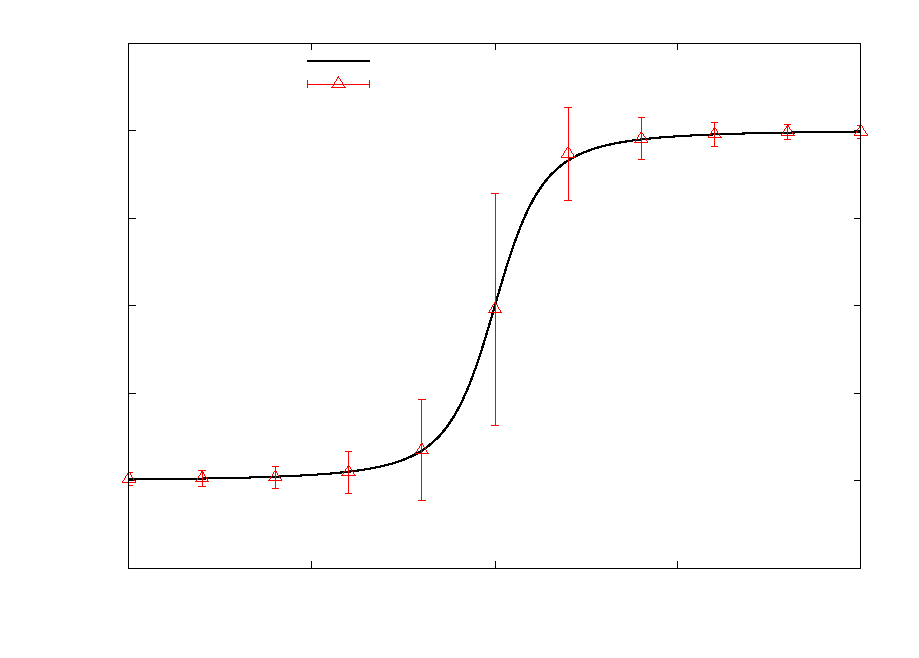
\includegraphics{magnetizationvaryingh}}%
    \gplfronttext
  \end{picture}%
\endgroup

		\caption{Magnetization for varying h, $N=16$, $2^{21}$ configurations sampled}
		\label{fig:magvarh}
	\end{figure}
	
\subsection{Varying N}

For varying $N$, our results for $h=1$ and $2^{21}$ sampled configurations are plotted together with the expectations in fig.~\ref{fig:magvarN}. Again our results follow the expectations pretty nicely: For $N=2$ the slope is a bit steeper than for the other configurations, $N=4$ is visibly a little bit steeper and below the curves for $N=8$ and $N=16$, which are on top of each other. Indeed, our measurements for $N=4,8,16$ lie pretty close to or even on top of each other, while the measurements for $N=2$ are visible below the other points. the errors of the measurements are larger for larger temperatures, and larger for smaller $N$, probably because of the size of the phase space.

	\begin{figure}[htbp]
		% GNUPLOT: LaTeX picture with Postscript
\begingroup
  \makeatletter
  \providecommand\color[2][]{%
    \GenericError{(gnuplot) \space\space\space\@spaces}{%
      Package color not loaded in conjunction with
      terminal option `colourtext'%
    }{See the gnuplot documentation for explanation.%
    }{Either use 'blacktext' in gnuplot or load the package
      color.sty in LaTeX.}%
    \renewcommand\color[2][]{}%
  }%
  \providecommand\includegraphics[2][]{%
    \GenericError{(gnuplot) \space\space\space\@spaces}{%
      Package graphicx or graphics not loaded%
    }{See the gnuplot documentation for explanation.%
    }{The gnuplot epslatex terminal needs graphicx.sty or graphics.sty.}%
    \renewcommand\includegraphics[2][]{}%
  }%
  \providecommand\rotatebox[2]{#2}%
  \@ifundefined{ifGPcolor}{%
    \newif\ifGPcolor
    \GPcolortrue
  }{}%
  \@ifundefined{ifGPblacktext}{%
    \newif\ifGPblacktext
    \GPblacktextfalse
  }{}%
  % define a \g@addto@macro without @ in the name:
  \let\gplgaddtomacro\g@addto@macro
  % define empty templates for all commands taking text:
  \gdef\gplbacktext{}%
  \gdef\gplfronttext{}%
  \makeatother
  \ifGPblacktext
    % no textcolor at all
    \def\colorrgb#1{}%
    \def\colorgray#1{}%
  \else
    % gray or color?
    \ifGPcolor
      \def\colorrgb#1{\color[rgb]{#1}}%
      \def\colorgray#1{\color[gray]{#1}}%
      \expandafter\def\csname LTw\endcsname{\color{white}}%
      \expandafter\def\csname LTb\endcsname{\color{black}}%
      \expandafter\def\csname LTa\endcsname{\color{black}}%
      \expandafter\def\csname LT0\endcsname{\color[rgb]{1,0,0}}%
      \expandafter\def\csname LT1\endcsname{\color[rgb]{0,1,0}}%
      \expandafter\def\csname LT2\endcsname{\color[rgb]{0,0,1}}%
      \expandafter\def\csname LT3\endcsname{\color[rgb]{1,0,1}}%
      \expandafter\def\csname LT4\endcsname{\color[rgb]{0,1,1}}%
      \expandafter\def\csname LT5\endcsname{\color[rgb]{1,1,0}}%
      \expandafter\def\csname LT6\endcsname{\color[rgb]{0,0,0}}%
      \expandafter\def\csname LT7\endcsname{\color[rgb]{1,0.3,0}}%
      \expandafter\def\csname LT8\endcsname{\color[rgb]{0.5,0.5,0.5}}%
    \else
      % gray
      \def\colorrgb#1{\color{black}}%
      \def\colorgray#1{\color[gray]{#1}}%
      \expandafter\def\csname LTw\endcsname{\color{white}}%
      \expandafter\def\csname LTb\endcsname{\color{black}}%
      \expandafter\def\csname LTa\endcsname{\color{black}}%
      \expandafter\def\csname LT0\endcsname{\color{black}}%
      \expandafter\def\csname LT1\endcsname{\color{black}}%
      \expandafter\def\csname LT2\endcsname{\color{black}}%
      \expandafter\def\csname LT3\endcsname{\color{black}}%
      \expandafter\def\csname LT4\endcsname{\color{black}}%
      \expandafter\def\csname LT5\endcsname{\color{black}}%
      \expandafter\def\csname LT6\endcsname{\color{black}}%
      \expandafter\def\csname LT7\endcsname{\color{black}}%
      \expandafter\def\csname LT8\endcsname{\color{black}}%
    \fi
  \fi
    \setlength{\unitlength}{0.0500bp}%
    \ifx\gptboxheight\undefined%
      \newlength{\gptboxheight}%
      \newlength{\gptboxwidth}%
      \newsavebox{\gptboxtext}%
    \fi%
    \setlength{\fboxrule}{0.5pt}%
    \setlength{\fboxsep}{1pt}%
\begin{picture}(8502.00,6008.00)%
    \gplgaddtomacro\gplbacktext{%
      \csname LTb\endcsname%
      \put(946,704){\makebox(0,0)[r]{\strut{}$-0.5$}}%
      \put(946,1964){\makebox(0,0)[r]{\strut{}$0$}}%
      \put(946,3224){\makebox(0,0)[r]{\strut{}$0.5$}}%
      \put(946,4483){\makebox(0,0)[r]{\strut{}$1$}}%
      \put(946,5743){\makebox(0,0)[r]{\strut{}$1.5$}}%
      \put(2483,484){\makebox(0,0){\strut{}$5$}}%
      \put(4240,484){\makebox(0,0){\strut{}$10$}}%
      \put(5997,484){\makebox(0,0){\strut{}$15$}}%
      \put(7754,484){\makebox(0,0){\strut{}$20$}}%
    }%
    \gplgaddtomacro\gplfronttext{%
      \csname LTb\endcsname%
      \put(176,3223){\rotatebox{-270}{\makebox(0,0){\strut{}magnetization}}}%
      \put(4591,154){\makebox(0,0){\strut{}N}}%
      \csname LTb\endcsname%
      \put(7118,1097){\makebox(0,0)[r]{\strut{}expectation}}%
      \csname LTb\endcsname%
      \put(7118,877){\makebox(0,0)[r]{\strut{}measurement}}%
    }%
    \gplbacktext
    \put(0,0){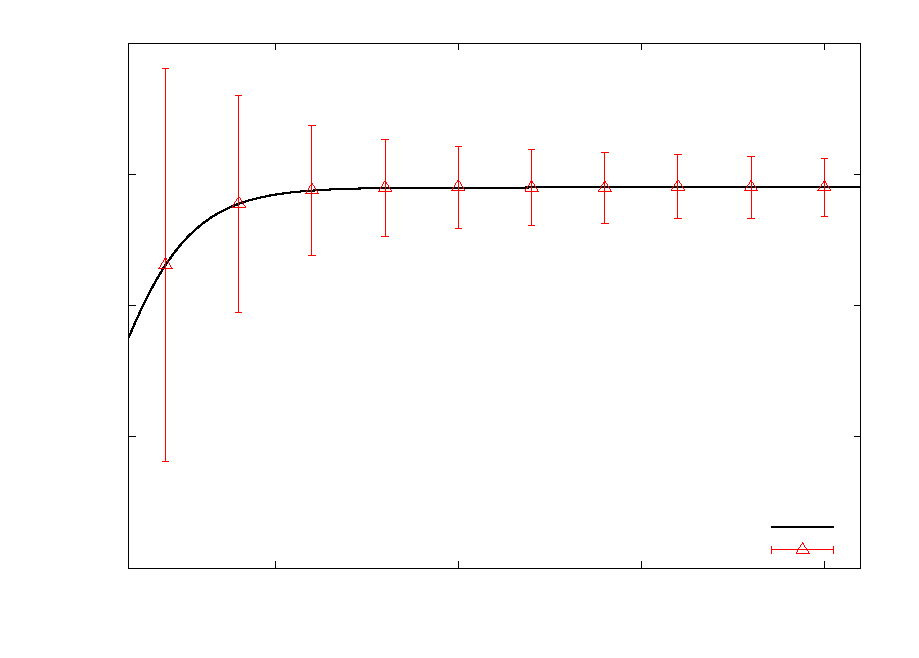
\includegraphics{magnetizationvaryingN}}%
    \gplfronttext
  \end{picture}%
\endgroup

		\caption{Magnetization for varying N, $h=1$, $2^{21}$ configurations sampled}
		\label{fig:magvarN}
	\end{figure}
	
\subsection{thermodynamical limit}

As seen above in fig.~\ref{fig:magvarN}, the expected magnetizations for $N=8$ and $N=16$ already lie on top of each other. We do not expect this to change for even bigger N, so our simulations with $N=16$ already reproduce the thermodynamical limit. 

We also see that Monte-Carlo simulation does not really make sense in this case: We sampled $2^{21}$ configurations, but even for $N=16$ this is a factor of $2^5$ larger than the entire phase space, which only contains $2^{16}$ possible configurations, and was solved in a few minutes. So in this case it would have been very easy and straightforward to sample the entire phase space. we have however seen that Monte-Carlo methods work and reproduce the expected solution quite nicely.
	
%	\begin{table}[htbp]
%		\centering
%		\begin{tabular}{l||l|l}
%			&Float&Double\\
%			\hline
%			&&\\
%			$h_{opt}$&$2.630\cdot10^{-3}$&$3.236\cdot10^{-6}$\\
%			$\delta_M$&$7.429\cdot10^{-9}$&$1.383\cdot10^{-17}$\\
%			$k$&$6.918\cdot10^{-5}$&$1.514\cdot10^{-8}$\\
%		\end{tabular} 
%		\caption{Ergebnisse für die Drei-Punkt-Ableitung} 
%		\label{tab:Drei-Punkt}
%	\end{table}
%	
	
\newpage	
\listoffigures
\printbibliography
\end{document}